\section{Three coherent regimes}
\label{sec:constructed}

The learned ladders fail persistence because their blocks are small compared with the distance a walker travels in $\tau$ steps.
This section shows that the failure is a property of those lenses, not of the program.
For three systems we write down nested lenses, explicit floors and explicit distance units, and prove that every requirement of \cref{def:coherence} holds in a joint limit in which substrate and lens are refined together.
The stage is $\tau=5$ throughout.
For the grid and the gasket the micro dynamics is exactly the lazy walk of \cref{sec:learned}; for the sphere it is a new family of reservoir chains.
In all three cases the lens is supplied by the structure of the substrate.
The results therefore establish that coherent geometric layers exist under these dynamics, and identify their limits; they do not show that such lenses can be found from an unlabelled kernel.

All three constructions rest on one mechanism.
\Cref{prop:closure-basic}(iii)--(iv) reduces closure and persistence to escape probabilities, and escape from a large block is rare because a walker must first reach the block boundary.
A probability floor below every positive macro weight leaves all edge costs untouched, and two-sided bounds on macro transition probabilities turn into two-sided bounds on the path metric.
\Cref{fig:defects-vs-cell} contrasts the resulting defects with those of the learned ladders.

\begin{figure}[t]
\centering
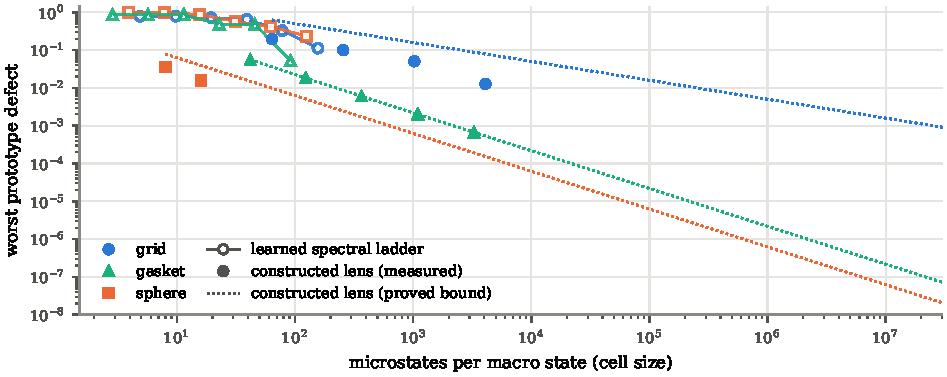
\includegraphics[width=\linewidth]{figures/fig_defects_vs_cell.pdf}
\caption{Worst prototype defect against block size. Hollow markers: the learned spectral ladders of \cref{sec:learned} (one marker per level). Filled markers: measured finite audits of the supplied lenses of this section. Dotted lines: the proved bounds $5/b$ (grid, block size $b^2$), $3\kappa/(V_s-3)$ (gasket, cell size $V_s$) and $5/(8V)$ (spherical reservoirs of volume $V$). For the reservoirs only the finest lens level is shown, where each macro state is a single reservoir and the cell size equals $V$.}
\label{fig:defects-vs-cell}
\end{figure}

\subsection{Grid: block lenses and an \texorpdfstring{$L^1$}{L1} limit}
\label{sec:grid}

Let the micro dynamics be the lazy walk on the open $N\times N$ grid of \cref{sec:substrates}, with $N=Mb$.
The block lens with width $b$ labels the site $(r,c)$ by $(\lfloor r/b\rfloor,\lfloor c/b\rfloor)$, giving an $M\times M$ array of blocks, and each prototype is uniform on its $b\times b$ block.
Lenses whose widths differ by an integer factor are nested by block containment.
Write $L(x,y)$ for the Manhattan distance between block indices.

\begin{theorem}[Coherent block lenses at stage five]
\label{thm:grid}
Let $b\ge8$ and $\tau=5$.
\begin{enumerate}[label=(\roman*)]
\item Every block has escape probability at most $5/b$; hence $\delta\le5/b$ and $\max_x s(x)\le5/b$.
\item Transitions between distinct blocks occur only between blocks that share a side (``cardinal'') or a corner (``diagonal''), with symmetrized weights
$\frac{1}{128b}\le W\le\frac5b$ on cardinal pairs and $\frac{1}{512b^2}\le W\le\frac{25}{b^2}$ on diagonal pairs.
\item With floor $\eta_b=1/(1024b^2)$ and threshold $0$, no edge is clipped, the macro graph is connected, and with $c_b=\log(128b)$ and $e=\log 640$,
\begin{equation}
(c_b-e)\,L(x,y)\;\le\;d_b(x,y)\;\le\;c_b\,L(x,y)\qquad\text{for all }x,y.
\end{equation}
\item In the declared unit $\lambda=Mc_b$, the normalized metric $\rho_b=d_b/(Mc_b)$ satisfies
$\max_{x,y}|\rho_b(x,y)-L(x,y)/M|\le 2\log640/\log(128b)$.
\item For nested lenses with widths $b_{\mathrm f}$ and $b_{\mathrm c}=2b_{\mathrm f}$, the normalized distortion is at most $2/M_{\mathrm f}+2\log640/\log(128b_{\mathrm f})+2\log640/\log(128b_{\mathrm c})$.
\item For a nested triple, the route mismatch on fine prototype inputs is at most $15/b_{\mathrm f}+5/b_{\mathrm m}$.
\end{enumerate}
\end{theorem}

\provenance{Written proof (\cref{app:grid-proof}). Lean: the step from escape to the closure defect on every microstate is \lean{closure_defect_le_macro_escape}. Exact and floating computation: complete ladders on grids of side $64$ and $128$ (finest $256$ blocks) check every macro edge against (ii) and every macro pair against (iii)--(v); tests compare the sparse staged computation with the dense original kernel.}

The escape bound comes from stationarity.
The stationary law of the open grid walk is proportional to vertex degree, a uniform block prototype is pointwise at most a fixed multiple of it, and this domination is preserved by the dynamics.
Each step therefore crosses the block boundary with probability at most $1/b$, and a union bound over five steps gives (i).
For (ii), a five-step walk with $b\ge8$ moves at most one block in each coordinate; explicit paths give the lower bounds and the need to start within five sites of the boundary gives the upper bounds.
The key consequence is (iii): a cardinal step costs about $\log b$ and a diagonal step about $2\log b$, so a cheapest protocol counts Manhattan steps.

\paragraph{Joint refinement and the limit.}
For $k\ge3$ put $t=2^k$, $N=4t^2$, and use the three nested lenses of widths $4t,2t,t$ (block arrays of side $t,2t,4t$).
Every requirement of \cref{def:coherence} holds: closure and prototype defects are at most $5/t$, every macro graph is connected, adjacent normalized distortions and route mismatches tend to zero, the number of blocks grows, and by (iii) the normalized diameter lies between $(1-e/c_b)\,2(M-1)/M$ and $2(M-1)/M$, so it tends to $2$.
Mapping each block to its centre in $[0,1]^2$ turns $L/M$ into exactly the $L^1$ distance between centres, and the centres form a net whose mesh tends to zero.
The normalized macro metrics therefore converge, uniformly on block centres and in the Gromov--Hausdorff sense~\cite{Gromov1999Metric}, to the unit square with the $L^1$ metric; quantitatively, the Gromov--Hausdorff distance is at most $\log640/\log(128b)+1/M$.

Two qualifications are part of the result.
First, the limit is not Euclidean.
The four corners of an $L^1$ square have side lengths $1$ and diagonals $2$, which violates~\eqref{eq:quadrilateral}; so coherence does not imply an inner-product geometry, and failure of Euclidean fit does not indicate a fractal.
Second, the convergence is slow and the units matter.
The readout error in (iv) decays only like $1/\log b$, and it is a conservative bound that is uninformative at the audited block widths, where the measured normalized readout errors are between $0.44$ and $1.06$ and the measured normalized distortions between $0.14$ and $0.30$.
In raw cost units, with the prescribed unit ratio, the distortion is multiplied by the fine unit $M_{\mathrm f}c_{b_{\mathrm f}}$ and need not vanish at all.

\subsection{Gasket: recursive cells and a fractal limit}
\label{sec:gasket}

\begin{figure}[t]
\centering
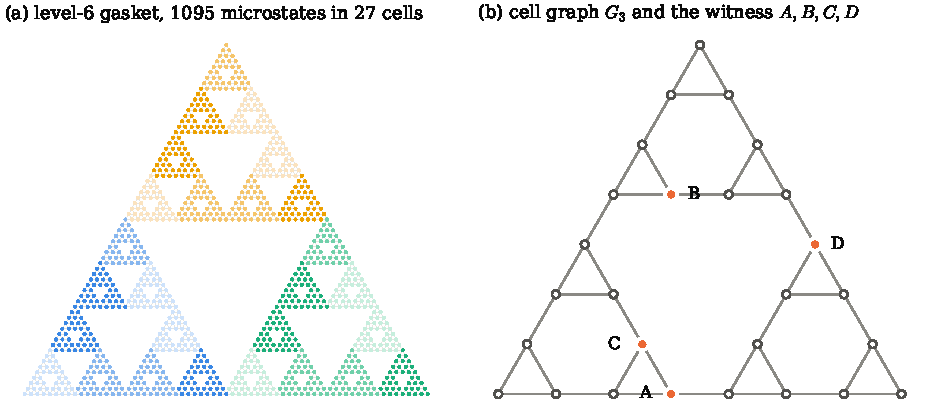
\includegraphics[width=\linewidth]{figures/fig_gasket_cells.pdf}
\caption{(a) The level-6 gasket graph ($1095$ microstates) partitioned into the $27$ recursive cells of level $3$; colours indicate cells (shades group them by their first address digit). (b) The cell contact graph $G_3$, whose unit-edge metric controls the macro metric. The four highlighted cells are the depth-3 prefixes of the limiting points $A,B,C,D$ of \cref{thm:gasket-limit}; their graph distances are $AB=CD=5$, $AC=1$, $BD=3$, $AD=BC=4$.}
\label{fig:gasket-cells}
\end{figure}

Let the micro dynamics be the lazy walk on the level-$\ell$ gasket graph, $\ell=s+m$ with $s\ge3$.
The recursive construction covers this graph by $3^m$ copies of the level-$s$ gasket, each with $V_s=(3^{s+1}+3)/2$ vertices; neighbouring copies share one corner vertex.
Assigning each shared vertex to the lexicographically first copy containing it gives disjoint fibres of sizes between $V_s-3$ and $V_s$, labelled by addresses of length $m$ over $\{0,1,2\}$ (\cref{fig:gasket-cells}a).
The ownership rule is nested, so deleting the last address digit is the containment map to the next coarser lens.
Prototypes are uniform on fibres.
Two cells are adjacent when their copies share a corner; the resulting cell contact graph $G_m$ consists of three copies of $G_{m-1}$ joined pairwise by single edges (\cref{fig:gasket-cells}b).
Let $D_m$ be its unit-edge graph metric.

\begin{theorem}[Coherent recursive cells at stage five]
\label{thm:gasket}
Let $s\ge3$, $m\ge1$, $\tau=5$ and $\kappa=11905/16384$.
\begin{enumerate}[label=(\roman*)]
\item For adjacent cells $K_{xy}=\kappa/n_x$, where $n_x$ is the fibre size; all other off-diagonal entries vanish.
\item Every escape probability, and hence $\delta$ and $\max_x s(x)$, is at most $3\kappa/(V_s-3)$.
\item With floor $\eta_s=\kappa/(2V_s)$ and threshold $0$, no edge is clipped, the macro graph is connected, and with $c_s=\log(V_s/\kappa)$ and $e_s=\log(V_s/(V_s-3))$,
$(c_s-e_s)D_m\le d_{s,m}\le c_sD_m$.
\item In the declared unit $2^mc_s$, the normalized metric $\rho_{s,m}=d_{s,m}/(2^mc_s)$ satisfies $\max|\rho_{s,m}-D_m/2^m|\le\epsilon_s\coloneqq e_s/c_s$.
\item Adjacent lenses on the same micro graph have parameters $(s,m)$ and $(s+1,m-1)$, and their normalized distortion is at most $2^{-m}+\epsilon_s+\epsilon_{s+1}$.
\item For a nested triple with fine and middle cell sizes $V_{\mathrm f}=V_s$ and $V_{\mathrm m}=V_{s+1}$, the route mismatch on fine prototype inputs is at most $\frac{32}{4(V_{\mathrm f}-3)-2}+\frac{3\kappa}{V_{\mathrm f}-3}+\frac{3\kappa}{V_{\mathrm m}-3}$.
\end{enumerate}
\end{theorem}

\provenance{Written proof (\cref{app:gasket-proof}). Exact computation: the interface constant $\kappa$ is the five-step crossing count $23810/8^5$ on the level-4 graph, and the contributing radius-five neighbourhood is the same for every $s\ge3$. Lean: \lean{closure_defect_le_macro_escape} (closure from escape) and \lean{gasket_staged_log_bracket} (cost bracket estimates). Exact and floating computation: complete ladders on gaskets of levels $6$, $7$ and $9$ (up to $29526$ microstates) check every bound; the worst finest prototype defects are $0.054$, $0.018$ and $0.0060$, and the route mismatches $0.0060$, $0.0020$ and $0.00066$.}

Statement (i) is the heart of the construction: since cell corners are at least $2^s\ge8$ steps apart, a five-step walk crosses at most one interface, and the probability flux across an interface is a universal constant independent of $s$.
For three-level ladders $(s+2,m-2)$, $(s+1,m-1)$, $(s,m)$ with $s,m\to\infty$, every requirement of \cref{def:coherence} holds: the number of cells grows and normalized diameters tend to one.

\paragraph{The limit space.}
Represent points by infinite addresses $a\in\{0,1,2\}^{\N}$ and put
\[
\delta_m(a,b)=D_m(a|_m,b|_m)/2^m,
\]
where $a|_m$ is the length-$m$ prefix.
Under last-digit deletion $r$ the graphs satisfy $|D_m(x,y)-2D_{m-1}(r(x),r(y))|\le1$, so $|\delta_{m+1}-\delta_m|\le2^{-(m+1)}$ and the $\delta_m$ converge uniformly.

\begin{theorem}[The gasket limit]
\label{thm:gasket-limit}
The limit $\delta=\lim\delta_m$ is a pseudometric on addresses with $|\delta-\delta_m|\le2^{-m}$. Identifying addresses at distance zero gives a compact metric space $(\mathcal G,\delta)$ of diameter $1$ with the following properties.
\begin{enumerate}[label=(\roman*)]
\item \emph{Self-similarity.} Prefixing a fixed word of length $j$ scales all distances by exactly $2^{-j}$, so $\mathcal G$ is covered by $3^j$ copies of itself scaled by $2^{-j}$.
\item \emph{Convergence of the Markov metrics.} For any $s_m\ge3$ with $s_m\to\infty$, the normalized metrics of \cref{thm:gasket} on micro level $s_m+m$ satisfy $|\rho_{s_m,m}-\delta|\le\epsilon_{s_m}+2^{-m}\to0$ on cell addresses.
\item \emph{Dimension.} With $d_f=\log3/\log2$ and $\mu$ the image of the uniform product measure, every ball satisfies $\tfrac13 r^{d_f}\le\mu(B_x(r))\le10\,r^{d_f}$ for $0<r<1$. Consequently $\dH\mathcal G=\log 3/\log 2$.
\item \emph{No local Hilbert approximation.} For every point $x$ and every $j\ge0$, there is no map from the ball $B_x(2^{-j})$ into a real inner-product space that changes all pairwise distances by at most $2^{-j}/16$.
\end{enumerate}
\end{theorem}

\provenance{Written proof (\cref{app:gasket-proof}), including the recursive graph laws, compactness, the measure bounds and the Hausdorff dimension argument. Lean: the strict scalar inequality behind (iv) is \lean{gasket_limit_quadrilateral_gap}, applied through \lean{no_hilbert_uniform_approximation}. Exact computation: the prefix distance formulas used in (iv) are checked for prefixes of length $3$ to $6$.}

Part (iv) uses four explicit points,
\begin{equation}
A=0\,1^{\infty},\qquad B=20\,1^{\infty},\qquad C=01\,2^{\infty},\qquad D=1\,2^{\infty},
\end{equation}
whose limiting distances are $\delta(A,B)=\delta(C,D)=\tfrac34$, $\delta(A,C)=\delta(B,D)=\tfrac14$ and $\delta(A,D)=\delta(B,C)=\tfrac12$.
These violate the quadrilateral inequality~\eqref{eq:quadrilateral}, and they still violate it with a strict gap of $15/128$ after every distance is moved by $1/16$ in the unfavourable direction.
By self-similarity, the prefix copy of length $j$ containing any given point $x$ lies in $B_x(2^{-j})$ and contains a copy of this configuration scaled by $2^{-j}$.
The finite Markov metrics carry the same obstruction: for $m\ge2$, a fixed six-cycle of $G_2$ remains isometrically embedded in $G_m$, and with the cost bracket of \cref{thm:gasket}(iii) its four-point witness excludes Hilbert fits to within one twelfth of its radius bound $3c_s$ (\lean{gasket_quadrilateral_gap}).
Because the finite witness and the limit approximation error are of comparable size, the limiting statement is proved from the fixed limiting points rather than transferred from finite witnesses.

The gasket limit is thus a genuinely fractal geometry obtained from the original micro dynamics: compact, self-similar, of non-integer Hausdorff dimension, and quantitatively non-Euclidean at every point and every dyadic scale.
It is a different object from the learned gasket ladder of \cref{sec:learned}, which still fails persistence, and the dimension proxies reported there are not estimates of $\log3/\log2$.

\subsection{Sphere: reservoir chains and a curved limit}
\label{sec:sphere}

The sphere $k$NN walk of \cref{sec:learned} has no natural nested lens, so the curved construction changes the micro dynamics.
Each macro point is a \emph{reservoir}: a cycle of $V\ge4$ microstates that holds with probability $5/8$ and moves to each cycle neighbour with probability $3/16$.
One state of each reservoir is its \emph{gateway}.
Given distinct points $q_1,\dots,q_n$ on the unit sphere with geodesic distance $d_S$, and a contact parameter $\beta>0$, gateways $i\neq k$ are linked with probability
\begin{equation}
Q_{ik}=\frac{2^{-\lceil\beta\, d_S(q_i,q_k)\rceil}}{8n},
\end{equation}
and each gateway's holding probability is reduced by its total contact rate.
In matrix form $P=I_n\otimes B+(Q-\operatorname{diag}(Q\one))\otimes G$, where $B$ is the cycle kernel and $G$ projects onto the gateway.
$P$ is stochastic, symmetric and connected, every diagonal entry is at least $\tfrac12$, and the stationary law is uniform.
The spherical geometry enters through the contact law: the substrate is designed to be spherical, just as the grid and gasket substrates are designed to be flat and self-similar.

The points $q_i$ come from nested cube meshes.
Each face of the cube $[-1,1]^3$ is divided into $2^{\ell}\times2^{\ell}$ cells, cell centres are projected radially to the sphere, and in one cell per face the representative is replaced by the face's axis point, so that the six axis points (and three mutually orthogonal ``landmarks'') belong to every mesh.
Dyadic parents give nested lenses.
For $r\ge5$, the system $\mathcal S_r$ has one reservoir per cell of level $r+2$ and lenses at levels $r$, $r+1$ and $r+2$, with
\begin{equation}
n_r=6\cdot4^{r+2},\qquad V_r=2^r,\qquad \beta_r=2^{r/2},\qquad t_r=\beta_r\log2,\qquad\tau=5.
\end{equation}
Every coarse fibre is a union of at most $16$ reservoirs, and prototypes are uniform on fibres.
Distances are measured in the declared unit $t_r$.

\begin{theorem}[Coherent spherical reservoirs]
\label{thm:sphere}
For every $r\ge5$, at all three lens levels of $\mathcal S_r$:
\begin{enumerate}[label=(\roman*)]
\item escape, $\delta$ and $\max_x s(x)$ are at most $5/(8V_r)$;
\item with threshold $0$ and the inactive floor $\eta=2^{-\lceil\beta_r\pi\rceil}/(256\,n_rV_r\cdot16)$, the macro graph is connected and, writing $r_x$ for the representative point of macro state $x$,
\begin{equation}
0\;\le\;\frac{d(x,y)}{t_r}-d_S(r_x,r_y)\;\le\;\epsilon_r\coloneqq 4\pi\sqrt2\,2^{-r}+\bigl(16+\log_2 6+3r\bigr)2^{-r/2};
\end{equation}
\item the normalized distortion between adjacent lens levels is at most $2\epsilon_r+2\varrho_r$, where $\varrho_r=2\pi\sqrt2\,2^{-r}$ bounds the cell radius;
\item the route mismatch is at most $5/(2V_r)$ on fine prototype inputs and at most $15a_r+5/(8V_r)$ on every micro point mass, where $a_r=O(2^{-r})$ bounds the contact rate of any gateway;
\item the normalized macro spaces converge in the Gromov--Hausdorff sense to the unit sphere with its geodesic metric; their diameters lie in $[\pi,\pi+\epsilon_r]$.
\end{enumerate}
\end{theorem}

\provenance{Written proof (\cref{app:sphere-proof}): killed-walk density bounds, first-contact flux with exponential moments, a per-edge baseline inequality, cube-mesh covering and packing estimates. Lean: \lean{likelihood_cost_exp_bracket}, \lean{Protocol.reference_le_cost} and \lean{weightedEdist_reference_bracket} in \lean{CoherentMetric.lean} pass probability brackets to the actual floored costs and to the protocol infimum; \lean{closure_defect_le_macro_escape} gives (i). Exact computation: at the finest lens (one reservoir per macro state) the stage-five macro kernel is $K_5=I+\frac1V\sum_{k=1}^5c_kA^k$ with $c=(5,\tfrac{7345}{1024},\tfrac{109}{16},\tfrac{31}{8},1)$ and $A=Q-\operatorname{diag}(Q\one)$, for every $V\ge4$; coarser kernels follow by uniform lifting and aggregation. Floating computation: two finite reservoir ladders with $768$ and $6144$ microstates, using smaller parameters than the family $\mathcal S_r$ (whose first member already has $3{,}145{,}728$ microstates), check the general finite-reservoir bounds under those parameters.}

The proof of (ii) is the delicate step.
An upper bound on $K_{xy}$ must allow walks that make several contacts, possibly back and forth, within five steps; this is handled by an exponential moment of the displacement, which grows by at most a factor $9/8$ per step.
A lower bound comes from a single contact followed by four holds.
Together they give, for every off-diagonal pair, $t\,d_S(r_x,r_y)\le c(x,y)\le t\,d_S(r_x,r_y)+2t\varrho_r+\log(256\,n_rV_r\cdot16)$; the additive term grows only linearly in $r$, so it is $o(t_r)$ and vanishes after division by the unit $t_r$. The lower bound holds for each edge separately, so coarsening errors cannot accumulate along long protocols.
Route coherence from every microstate, not just from prototypes, needs a packing estimate: no gateway has many reservoirs nearby, so the contact rate $a_r$ from any single microstate is small.

The construction keeps the stage, the likelihood cost, the shortest-path readout and all coherence gates, and changes the micro dynamics and the lens family; we do not claim that these changes are necessary.
Its parameters are tuned to the limit: the finite audits use small volumes and contact parameters outside the family $\mathcal S_r$, at which the metric error bound is far from small, so they check the implementation rather than illustrate convergence.
The limits involve probabilities of order $2^{-\beta_r\pi}$, which double-precision arithmetic cannot represent for large $r$; the family is a mathematical construction, not a scalable simulation.
\Cref{sec:transport-repair} shows that its metrics carry enough information to recover spherical curvature.
